\section{A Primer on Neural Networks\skipthis}
\thispagestyle{plain}

We have already seen that we can write logistic and multiclass
classification in a \textit{electrical engineering style} diagram.
This can analogously be done for linear regression.

\subsection{The final layer of a neural network for classification and regression}
Assume a linear model
\begin{equation}
    \hat{y}_i = \beta_0 + \sum_{j=1}^{p} \beta_j x_{ij} = 1( \beta_0 + \sum_{j=1}^{p} \beta_j x_{ij} )
\end{equation}
where $1(\cdot)$ is the identity function. We can illustrate this in the same
style, we used for logistic regression, as illustrated in figure
\ref{fig:lin_class_electrical}.

\begin{figure}[!htb]
    \centering
    \includesvg[width=0.95\textwidth]{figures/lin_class.svg}
    \caption{Electrical engineering style diagrams.}
    \label{fig:lin_class_electrical}
\end{figure}

A comparison between classification and regression is given in table \ref{tab:classification_vs_regression}.

% make 2 table with three columns, one for classification and one for regression
% the rows are data, model, loss
\begin{table}[!htb]
    \centering
    \begin{tabular}{|p{0.08\textwidth}|p{0.43\textwidth}|p{0.43\textwidth}|}
        \hline
        & \textcolor{blue1}{Regression} & \textcolor{blue1}{Classification} \\
        \hline
        Data & (Multiple) Continuous output(s) $\vec{y}$
        \begin{equation*}
            \begin{gathered}
                \{ \vec{x}_i, \vec{y}_i \}_{i=1}^{N} \\
                \vec{x}_i \in \mathbb{R}^p, \vec{y}_i \in \mathbb{R}^K
            \end{gathered}
        \end{equation*} & 1-hot class label $\vec{c} \in \{0,1\}^K$
        \begin{equation*}
            \begin{gathered}
                \{ \vec{x}_i, \vec{c}_i \}_{i=1}^{N} \\
                \vec{x}_i \in \mathbb{R}^p, \vec{c}_i \in \{0,1\}^K, \sum_{k=1}^{K} c_{ik} = 1
            \end{gathered}
        \end{equation*} \\
        \hline
        Model & \begin{equation*}
            \vec{\hat{y}} = \mat{W} \vec{x}
        \end{equation*} &
        \begin{equation*}
            \vec{\hat{c}} = \operatorname{softargmax}(\mat{W} \vec{x})
        \end{equation*} \\
        \hline
        Loss & Squared residuals loss \begin{equation*}
            \mathcal{L}(\vec{y}, \vec{\hat{y}}) = \frac{1}{N} \sum_{i=1}^{N} \left( \vec{y}_i - \vec{\hat{y}}(\vec{x}_i) \right)^2
        \end{equation*} &
        Cross-entropy loss \begin{equation*}
            \mathcal{L}(\vec{c}, \vec{\hat{c}}) = - \frac{1}{N} \sum_{i=1}^{N} \sum_{k=1}^{K} \vec{c}_i^T \log(\vec{\hat{c}}(\vec{x}_i))
        \end{equation*} \\
        \hline
    \end{tabular}
    \caption{Aim in both cases: Find $\mat{W}$ that minimizes the loss. An offset is achieved by a $1$ entry in the $\vec{x}$ vector.
    We are in a supervised setting with supervisions $\vec{y}$ and $\vec{c}$ respectively.}
    \label{tab:classification_vs_regression}
\end{table}

\subsection{Adding hidden layers - path to a neural network}
\textbf{Why should we add more layers?:} We have previously seen, 
that by the function counting theorem,
projection to higher dimensions can make a problem linearly separable.
In the context of linear regression a basis expansion helped us to fit
more complex non-linear functions.

We can also remember the generalized linear model, where we use a 
mean function $g$ applied to a linear model, to have a mean prediction
\begin{equation}
    \mu_i = g(\vec{\beta}^T \vec{x}_i)
\end{equation}

\idea{Construct a whole network of such nodes, where the outputs of one layer are fed forward into
the next layer, first an input layer, then \textit{hidden layers} and finally the output layer, different
for classification and regression, as discussed. This is illustrated in figure \ref{fig:nn_illu}.}

\begin{figure}[!htb]
    \centering
    \includesvg[width=0.95\textwidth]{figures/nn_illu.svg}
    \caption{A neural network.}
    \label{fig:nn_illu}
\end{figure}

Later our central question will be, what weights to choose to minimize the loss.

\subsubsection{On the choice of activation function}
Different activation functions are illustrated in figure \ref{fig:activation_functions}.
Based on their different shapes, they give different outputs, e.g. different
decision boundaries in classification or different fits in regression. Their properties
also effect the training, so finding appropriate weights and biases (the offset terms).

\begin{figure}[!htb]
    \centering
    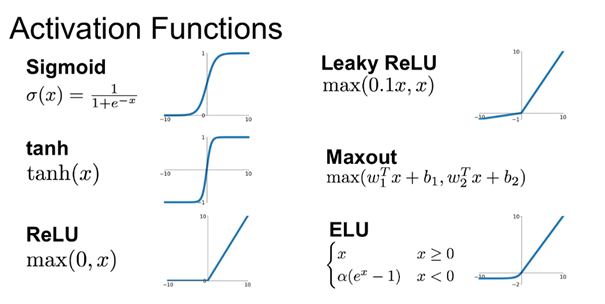
\includegraphics[width=0.8\textwidth]{figures/activation_functions.png}
    \caption{Different activation functions.}
    \label{fig:activation_functions}
\end{figure}

\subsubsection{Neural Network are universal function approximators}
\greenbox{By a single hidden layer, a neural network with finite number of nodes can
approximate any continuous function on a compact set to arbitrary precision.}

Consider a continuous, non-constant bounded activation function
\begin{equation}
    g(z) \rightarrow \begin{cases}
        1 & z \rightarrow \infty \\
        0 & z \rightarrow -\infty
    \end{cases}
\end{equation}
then any continuous $f$, here on $I_p = [0,1]^p$, can be approximated by a finite size
neural network

\begin{equation}
    \forall \epsilon > 0, \forall f \in C(I_p), \exists \text{finite sum } F_\vec{\theta}(\vec{x}) = \sum_{i=1}^{N} \theta_i g(\vec{w}_i^T \vec{x} + w_{0i}): \forall \vec{x} \in I_p, |f(\vec{x}) - F_\vec{\theta}(\vec{x})| < \epsilon
\end{equation}

\subsubsection{Neural Networks and Algorithmic modeling}
A neural network $F_\vec{\theta}$ (parameters $\vec{\theta}$) is deterministic universal
approximator. When we use a neural network to predict the relationship between input $\vec{x}$
and output $\vec{y}$, we directly model the relation between input and output, it is an algorithmic
modeling approach (as random forests), different from a data modeling approach, where we would assume a certain
model that has generated the data and some noise term \citep{breiman01} (and usually predict $E[y|x]$ under the model).

While in algorithmic modeling, we are not limited by a certain, possibly wrong model, interpretability
is usually limited.

The cultures of modelling are illustrated in figure \ref{fig:modelling_cultures}.

\begin{figure}[!htb]
    \centering
    \includesvg[width=0.95\textwidth]{figures/modelling_cultures.svg}
    \caption{Different cultures of modelling.}
    \label{fig:modelling_cultures}
\end{figure}

\subsection{Training of a neural network}

\subsubsection{Problem statement of training NNs}
Let us consider a network with parameters collected into a vector $\vec{W}$.
For an observation $\vec{x}_i$ the network output is $f(\vec{x}_i, \vec{W})$.
The supervision in the training set is $\vec{y}_i$, $\mathcal{D} = \{ (\vec{x}_i, \vec{y}_i) \}_{i=1}^{N}$.

We can formulate the training problem as

\begin{equation}
    \vec{\hat{W}} = \argmin_{\vec{W}} \mathcal{Q}(\vec{W}) = \argmin_{\vec{W}} \sum_{i\in \mathcal{D}} \text{loss}(f(\vec{x}_i, \vec{W}), \vec{y}_i) + \Omega_\text{architecture}(\vec{W}) + \Omega_\text{output}(f(\vec{x}_i, \vec{W}))
\end{equation}

with regularizations $\Omega_\text{architecture}$ and $\Omega_\text{output}$.

In the regression setting the loss would be
\begin{equation}
    \text{loss}(f(\vec{x}_i, \vec{W}), \vec{y}_i) = \left( f(\vec{x}_i, \vec{W}) - \vec{y}_i \right)^2
\end{equation}

\subsubsection{Stochastic Gradient Descent for minimizing the loss}
We use gradient descent for the parameter estimates.
\subsubsubsection{Normal gradient descent}
Starting from an initial guess $\vec{W}^{(0)}$, we update the parameters by
\begin{equation}
    \vec{W}^{(t)}=\vec{W}^{(t-1)}-\alpha \vec{g}^{(t)}, \quad \vec{g}^{(t)}=\left.\frac{\partial Q(\vec{W})}{\partial \vec{W}}\right|_{\vec{W}^{(t-1)}}, \quad \text { learning rate } \alpha
\end{equation}
where the loss is calculated over the whole training dataset
\begin{equation}
    Q(\vec{W})=\sum_{i \in \mathcal{D}} \text { loss }\left(f\left(\vec{x}_{i}, \vec{W}\right), \vec{y}_{i}\right)
\end{equation}

\subsubsubsection{Stochastic gradient descent}
We introduce stochasticity (agains local minima) and reduce the length of the summation
by drawing an index subset $k^\star \subset 1, \ldots, N$ so a corresponding mini-batch
dataset $\mathcal{D}^\star \subset \mathcal{D}$

\begin{equation}
    Q(\vec{W})=\sum_{i \in \mathcal{D}^\star} \text { loss }\left(f\left(\vec{x}_{i}, \vec{W}\right), \vec{y}_{i}\right)
\end{equation}

\subsubsection{How to compute the gradients? | backpropagation}
\subsubsubsection{Gradient we want to compute}
At each update step in gradient descent, we want to compute
\begin{equation}
    \frac{\partial Q(\vec{W})}{\partial \vec{W}} = \sum_{i \in \mathcal{D}^\star} \frac{\partial \text{loss}\left(f\left(\vec{x}_{i}, \vec{W}\right), \vec{y}_{i}\right)}{\partial \vec{W}}
\end{equation}
So to update our weights fromt $W^{(t-1)}$ to $W^{(t)}$ we need to compute

\begin{equation}
    \left.\frac{\partial \operatorname{loss}\left(\vec{y}_i, \vec{f}\left(\vec{x}_i, \vec{W}\right)\right)}{\partial \vec{W}}\right|_{\vec{W}^{(t-1)}}=\left(\begin{array}{c}
    \left.\frac{\partial \mathcal{Q}(\vec{W})}{\partial W_1}\right|_{\vec{W}^{(t-1)}} \\
    \left.\frac{\partial \mathcal{Q}(\vec{W})}{\partial W_2}\right|_{\vec{W}^{(t-1)}} \\
    \vdots \\
    \left.\frac{\partial \mathcal{Q}(\vec{W})}{\partial W_j}\right|_{\vec{W}^{(t-1)}} \\
    \left.\frac{\partial \mathcal{Q}(\vec{W})}{\partial W_{\mathfrak{P}}}\right|_{\vec{W}^{(t-1)}}
    \end{array}\right)
\end{equation}

on each training sample $\{ \vec{x}_i,\vec{y}_i \}$ in the minibatch, to later sum over the minibatch

\subsubsubsection{Why can't we use finite differencing?}
The derivative with respect to one weight can be approximated by
\begin{equation}
    \frac{\partial Q(\vec{W})}{\partial W_k}=\frac{\operatorname{loss}\left(\vec{y}_i, \vec{f}\left(\vec{x}_{i^{\prime}}\left(W_1, \ldots, W_k+\Delta W, \ldots, W_M\right)\right)\right)-\operatorname{loss}\left(\vec{y}_{i^{\prime}}, \vec{f}\left(\vec{x}_i, \vec{W}\right)\right)}{\Delta W}
\end{equation}
\problem{
    \begin{itemize}
        \item Per training data sample we would need as many computations of the loss, so forward passes
        though the network, as there are weights - infeasible.
        \item The finite difference approximation is not exact.
    \end{itemize}
}

\subsubsubsection{Backpropagation to the help}
\paragraph*{Neural Network as a composition of functions} Let
\begin{itemize}
    \item $L$ be the number of layers in our network
    \item $\vec{x}$ be our sample feature with target output $\vec{y}$
\end{itemize}
Let $\vec{a}^{(l-1)}$ be the input to the $l$-th layer, which consists of
\begin{itemize}
    \item the matrix containing the weights of the $l$-th layer $\mat{W}^{(l)}$ with elements
    $w_{j,k}^{(l)}$ sometimes denoted $w_k^{l,j}$. $w_{j,k}^{(l)}$ is the weight from the $k$-th node in the $l-1$-th layer to the $j$-th node in the $l$-th layer.
    After weighting, we get $\vec{z}^{(l)} = \mat{W}^{(l)} \vec{a}^{(l-1)}$.
    \item the activation functions $\vec{h}^{(l)}$ of the $l$-th layer
\end{itemize}
Then the output of the $l$-th layer is
\begin{equation}
    \vec{a}^{(l)} = \vec{h}^{(l)}(\vec{z}^{(l)}) = \vec{h}^{(l)}(\mat{W}^{(l)} \vec{a}^{(l-1)})
\end{equation}

The output of our whole network can then be written as

\begin{equation}
    \vec{f}(\vec{x}, \vec{W}) = \vec{a}^{(L)} = \vec{h}^{(L)}(\mat{W}^{(L)} \vec{a}^{(L-1)}) = \vec{h}^{(L)}(\mat{W}^{(L)} \vec{h}^{(L-1)}(\mat{W}^{(L-1)} \dots \vec{h}^{(1)}(\mat{W}^{(1)} \vec{x})))
\end{equation}

\paragraph*{Chain rule to the help for efficiently calculating gradients} Consider the
exemplary network in figure \ref{fig:nn_simple}.

\begin{figure}[!htb]
    \centering
    \includesvg[width=0.95\textwidth]{figures/nn_simple.svg}
    \caption{A simple neural network.}
    \label{fig:nn_simple}
\end{figure}

\bluebox{\textbf{Aim:} We want to calculate the partial derivatives of $\text{loss}(f(\vec{x}, \vec{W}), \vec{y})$ with respect to for instance $w_{1,1}^{(1)} = w_1^{1,1}$ and $w_{1,2}^{(1)} = w_2^{1,1}$ of the first layer.}

Chain rule gives us

\begin{equation}
    \begin{aligned}
    & \frac{\partial \operatorname{loss}\left(\vec{y}, \sigma\left(\mat{W}^{(2)} \vec{\vec{h}}^{(1)}\left(\mat{W}^{(1)} \vec{x}\right)\right)\right)}{w_{1,1}^{(1)}}=\frac{\partial \operatorname{loss}(\ldots)}{\partial \sigma(\ldots)} \frac{\partial \sigma(\ldots)}{\partial \vec{h}^{(1)}(\ldots)} \frac{\partial \vec{h}^{(1)}(\ldots)}{\partial \vec{W}^{(1)} \vec{x}} \frac{\partial \mat{W}^{(1)} \vec{x}}{\partial w_{1,1}^{(1)}} \\
    & \frac{\partial \operatorname{loss}\left(\vec{y}, \sigma\left(\mat{W}^{(2)} \vec{h}^{(1)}\left(\mat{W}^{(1)} \vec{x}\right)\right)\right.}{w_{1,2}^{(1)}}=\frac{\partial \operatorname{loss}(\ldots)}{\partial \sigma(\ldots)} \frac{\partial \sigma(\ldots)}{\partial \vec{h}^{(1)}(\ldots)} \frac{\partial \vec{h}^{(1)}(\ldots)}{\partial \mat{W}^{(1)} \vec{x}} \frac{\partial \mat{W}^{(1)} \vec{x}}{\partial w_{1,2}^{(1)}}
    \end{aligned}
\end{equation}

\begin{itemize}
    \item calculating this from left to right is called \textit{reverse mode differentiation} or \textit{backpropagation}
    \item calculating this from right to left is called \textit{forward mode differentiation}
\end{itemize}

\greenbox{Note that when going from left to right, the partial derivatives of the example only differ in the last term.}

\bluebox{For a system with few inputs and many outputs, we prefer the forward mode, for a system with many inputs
(the weights are also kind of inputs to the system), but few outputs, we prefer the reverse mode.}

\subsubsubsection{Intermezzo: Automatic differentiation}
Let us better understand the concept of derivatives propagating
forwards and backwards.
\paragraph*{On the derivatives of composite functions} Consider we have a function
$\vec{f}: \mathbb{R}^n \rightarrow \mathbb{R}^m$ and we want to calculate
\begin{equation}
    \frac{\partial f_i}{\partial x_i}
\end{equation}
Now consider $f$ is a \textbf{composite function}
\begin{equation}
    \vec{f}(\vec{x}) = \vec{h} \circ \vec{g}(\vec{x}) = \vec{h}(\vec{g}(\vec{x})), \quad \vec{x} \in \mathbb{R}^n, \vec{g}: \mathbb{R}^n \rightarrow \mathbb{R}^p, \vec{h}: \mathbb{R}^p \rightarrow \mathbb{R}^m
\end{equation}
then the chain rule is given by
\begin{equation}
    \frac{\partial f_i}{\partial x_j} = \sum_{k=1}^{p} \frac{\partial h_i}{\partial g_k} \frac{\partial g_k}{\partial x_j}
\end{equation}
so intuively to see how wiggling at $x_j$ changes $f_i$, we look how wiggling at $x_j$ affects the
intermediate $g_k$ and how wiggling at $g_k$ affects $f_i$ and chain the result. The point of
evaluation is the $x_j$ where we wiggle around.

\paragraph*{Writing a function as a computational graph} 
Consider the computational graph in figure \ref{fig:comp_graph}.

\begin{figure}[!htb]
    \centering
    \includesvg[width=0.95\textwidth]{figures/comp_graph.svg}
    \caption{A computational graph.}
    \label{fig:comp_graph}
\end{figure}

\bluebox{\textbf{Aim:} At a given $\vec{x}$, we want to calculate
\begin{equation}
    \begin{gathered}
        \left. \partial_{x_1} f_1 \right|_{\vec{x} = \vec{x}}, \quad \left. \partial_{x_2} f_1 \right|_{\vec{x} = \vec{x}} \\
        \left. \partial_{x_1} f_2 \right|_{\vec{x} = \vec{x}}, \quad \left. \partial_{x_2} f_2 \right|_{\vec{x} = \vec{x}}
    \end{gathered}
\end{equation}}

At given $\vec{x}$ and \textit{wiggling} $\vec{\xi} = \begin{pmatrix}
    x_1' & x_2'
\end{pmatrix}$ we can calculate the directional derivative
\begin{equation}
    \frac{\partial f_1}{\partial x_1} \xi_1 + \frac{\partial f_1}{\partial x_2} \xi_2
\end{equation}
by a forward pass through the graph, as illustrated in figure \ref{fig:comp_graph_dir_deriv}.

\begin{figure}[!htb]
    \centering
    \includesvg[width=0.95\textwidth]{figures/forward_pass.svg}
    \caption{Forward pass through the computational graph.}
    \label{fig:comp_graph_dir_deriv}
\end{figure}

For $\vec{\xi} = \begin{pmatrix}
    1 & 0
\end{pmatrix}$ we calculate $\partial_{x_1} \vec{f}$ derivatives of both outputs with
respect to a change in one input variable in one forward AD (automatic differentiation) pass. 

\greybox{Computationally this can just be fone by passing a dual number through $\vec{f}$}

\paragraph*{Backpropagation} Here we go the other way around, as
illustrated in figure \ref{fig:comp_graph_backprop}.

\begin{figure}[!htb]
    \centering
    \includesvg[width=0.95\textwidth]{figures/backprop.svg}
    \caption{Backpropagation through the computational graph.}
    \label{fig:comp_graph_backprop}
\end{figure}

\subsubsubsection{Error backpropagation in a neural network}
We have seen that based on the chain rule, we can efficiently calculate
gradients of functions with lots of inputs and few outputs - e.g. lots of weights,
which are also inputs, and one loss function.

\paragraph*{What errors are propagating?}
Remember that the neurons output is given by $h_j^{(l)}(z_j^{(l)})$.

Imagine there is a little benign demon that can slightly tweak $z_j^{(l)}$.

Consider the quantity
\begin{equation}
    \delta_j^{(l)} = \frac{\partial \mathcal{Q}(\vec{W})}{\partial z_j^{(l)}}
\end{equation}

Let us call $\vec{\delta}^{(l)}$ the error in the $l$-th layer, with $\delta_j^{(l)}$
being the error of the $j$-th neuron in the $l$-th layer.

\textbf{Why is $\delta_j^{(l)}$ called an error?:} If $\vec{\delta}^{(l)}$ is small 
our daemon can't improve the loss much by tweaking $z_j^{(l)}$ but if $\vec{\delta}^{(l)}$ is large,
there is lots of room for improvement.

The error in the output layer $L$ is given by

\begin{equation}
    \delta_j^{(L)} = \frac{\partial \text{loss}}{\partial z_j^{(L)}} = \frac{\partial \text{loss}}{\partial a_j^{(L)}} \frac{\partial a_j^{(L)}}{\partial z_j^{(L)}}
\end{equation}

Consider the quadratic loss $\text{loss} = \frac{1}{2} \sum_{j=1}^{m} \left( a_j^{(L)} - y_j \right)^2$ 
(for supervision $\vec{y} \in \mathbb{R}^m$) and as typical for regression, the output activation
function, different from the hidden layers, is the identity function $a_j^{(L)} = z_j^{(L)}$.

Then we have

\begin{equation}
    \delta_j^{(L)} = a_j^{(L)} - y_j
\end{equation}

\bluebox{So in the regression setting $\delta_j^{(L)}$ is quite literally the error between the output of the
neuron and the wanted output.}

By the chain rule, this error is propagated backwards by (\textbf{error backpropagation})

\begin{equation}
    \delta_j^{(l)}=\frac{\partial \operatorname{loss}}{\partial z_j^{(l)}}=\sum_{k \in \operatorname{children}\left(v_i\right)} \frac{\partial \operatorname{loss}}{\partial z_k^{(l+1)}} \frac{\partial z_j^{(l+1)}}{\partial z_j^{(l)}}=\left.\frac{\partial h_j^{(l)}}{\partial z}\right|_{z_j^{(l)}} \sum_{k \in \operatorname{children}\left(v_i\right)} \delta_k^{(l+1)} w_{k j}^{(l+1)}
\end{equation}

And the \textbf{partial derivatives of interest} are given by

\begin{equation}
    \frac{\partial \operatorname{loss}(\vec{y}, \vec{f}(\vec{x}, \vec{W}))}{\partial w_{j, k}^{(l)}}=a_k^{(l-1)} \delta_j^{(l)}
\end{equation}

\yellowbox{\textbf{When does a weight learn slowly?}: A weight will change only little
in the gradient descent steps, if \begin{itemize}
    \item the input to the neuron is small, $a_k^{(l-1)}$ is small
    \item the output has saturated, $\delta_j^{(l)}$ is small by (see backpropagation formula) $\left.\frac{\partial h_j^{(l)}}{\partial z}\right|_{z_j^{(l)}}$ being small
\end{itemize}}

\bluebox{\textbf{Backpropagation algorithm:}\begin{enumerate}
    \item For each training sample
    \begin{itemize}
        \item Feedforward: Compute $\vec{a}^{(l)}$ and $\vec{z}^{(l)}$ for all layers
        \item Output errors: calculate $\vec{\delta}^{(L)}$
        \item Backpropagate errors: calculate $\vec{\delta}^{(l)}$ for all layers, starting
        from the output layer, using the previous results on those from the feedforward pass along the way
        \item Compute the gradients:
        \begin{equation*}
            \frac{\partial \operatorname{loss}(\vec{y}, \vec{f}(\vec{x}, \vec{W}))}{\partial w_{j, k}^{(l)}}=a_k^{(l-1)} \delta_j^{(l)}
        \end{equation*}
    \end{itemize}
    \item Update the weights based on gradient descent using the average of the gradients over the minibatch
\end{enumerate}}

\subsubsubsection{Problem in training deep networks: Exploding and vanishing gradients}
Reconsider the error-backpropagation formula
\begin{equation}
    \delta_j^{(l)}=\frac{\partial \operatorname{loss}}{\partial z_j^{(l)}}=\sum_{k \in \operatorname{children}\left(v_i\right)} \frac{\partial \operatorname{loss}}{\partial z_k^{(l+1)}} \frac{\partial z_j^{(l+1)}}{\partial z_j^{(l)}}=\left.\frac{\partial h_j^{(l)}}{\partial z}\right|_{z_j^{(l)}} \sum_{k \in \operatorname{children}\left(v_i\right)} \delta_k^{(l+1)} w_{k j}^{(l+1)}
\end{equation}
Which is a multiplicative chain (with summations) through the network starting from 
the output layer. So, for deep networks
\begin{equation}
    \left| \frac{\partial z_j^{(l+1)}}{\partial z_j^{(l)}} \right| \rightarrow \begin{cases}
        > 1 & \text{exploding gradients} \\
        < 1 & \text{vanishing gradients}
    \end{cases}
\end{equation}

But we sometimes want to use deep networks as they might be more expressive (e.g.
because sublayers learn simpler patterns).

\greenbox{\textbf{ReLU against exploding and vanishing gradients}: For a ReLU activation function
\begin{equation}
    \text{ReLU for } z_j^{(l)} > 0: \left. \frac{\partial h_j^{(l)}}{\partial z} \right|_{z_j^{(l)}} = 1
\end{equation}
But we have a problem with vanishing gradients for $z_j^{(l)} < 0$ - so maybe use a leaky ReLU.
Another alleviation might be layerwise pretraining.
}

\subsection{Outlook}
\begin{itemize}
    \item use NN architectures reflecting the problem symmetry
    \item bake in physical knowledge into the loss, regularizing on a differential equation
    \item ...
\end{itemize}


\pagebreak